\def\mySecNum{2.5}
\mySection{\mySecNum~Summary of forward and option positions}
%-------------- start slide -------------------------------%{{{ 1
\begin{frame}[fragile]
\begin{eqnarray*}
	\left\{\text{long},\text{short}\right\} & \times & \left\{\text{forward}, \text{call}, \text{put}\right\} \\[1.2em]
                                          & |  |   &
\end{eqnarray*}
\begin{align*}
	\text{six positions}\hspace{3em}
\end{align*}
\end{frame}
%-------------- end slide -------------------------------%}}}
%-------------- start slide -------------------------------%{{{ 1
\begin{frame}[fragile,t]

\begin{center}
	Maximum possible profit and loss at maturity for \\
	$\left\{\text{long},\text{short}\right\} \times \left\{\text{forward}, \text{call}, \text{put}\right\}$
	\mySeparateLine
	\bigskip

	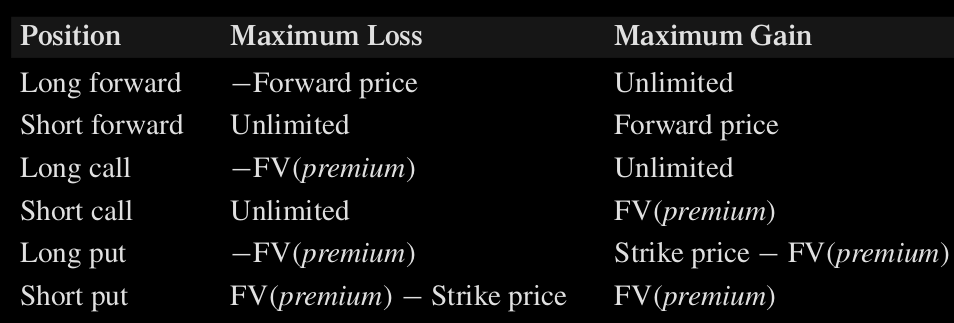
\includegraphics[scale=0.3]{figs/Table2-5.png}\footnote{$FV(\cdot)$ denotes the function that returns the future value.}
\end{center}
\end{frame}
%-------------- end slide -------------------------------%}}}
%-------------- start slide -------------------------------%{{{ 1
\begin{frame}[fragile]
\begin{center}
	Profit diagrams for \\
	$\left\{\text{long},\text{short}\right\} \times \left\{\text{forward}, \text{call}, \text{put}\right\}$
	\mySeparateLine
	\bigskip

	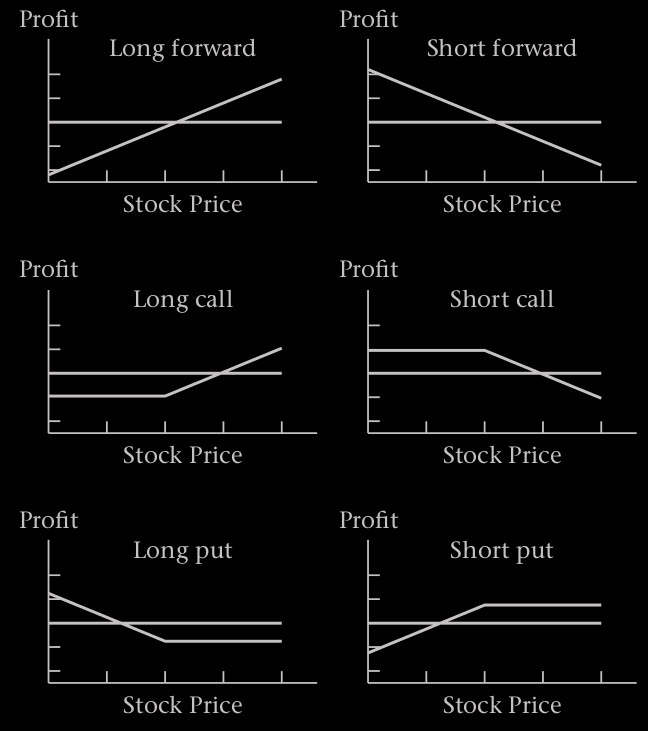
\includegraphics[scale=0.27]{figs/Figure-2-14.png}
\end{center}
\end{frame}
%-------------- end slide -------------------------------%}}}
%-------------- start slide -------------------------------%{{{ 1
\begin{frame}[fragile]
\begin{center}
	Summary of positions for \\
	$\left\{\text{long},\text{short}\right\} \times \left\{\text{forward}, \text{call}, \text{put}\right\}$
	\mySeparateLine
	\bigskip

	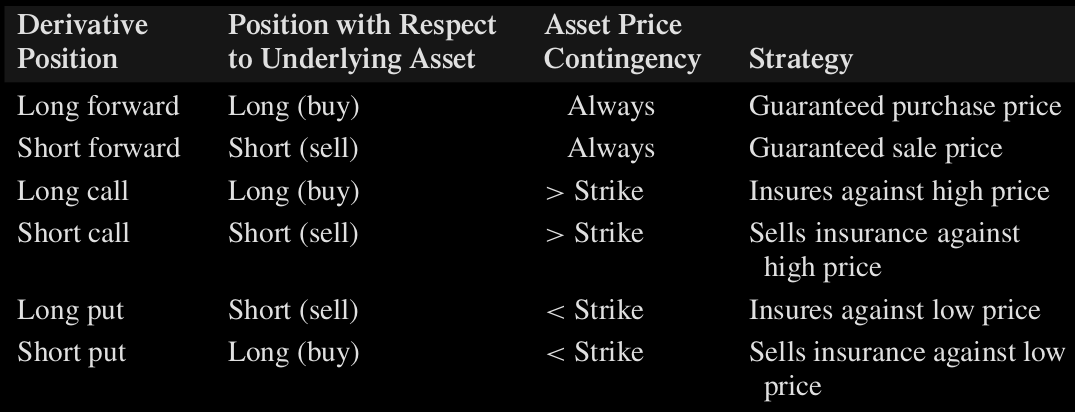
\includegraphics[scale=0.25]{figs/Table-2-7.png}
\end{center}
\end{frame}
%-------------- end slide -------------------------------%}}}
